% ============================================================================
%  Выпускная квалификационная работа (бакалаврская работа)
%  Володин М. В., ЛФИ МФТИ, 2026
%  Сборка: pdflatex thesis.tex (дважды, для оглавления и ссылок)
% ============================================================================
% Некоторые файлы лежат рядом с этим .tex (пакетный менеджер MiKTeX недоступен, поэтому класс подключён локально).
\documentclass[14pt,a4paper]{extreport}

\usepackage[utf8]{inputenc}
\usepackage[T2A]{fontenc}
\usepackage[russian]{babel}
\usepackage{tempora}            % Times-подобный шрифт с поддержкой кириллицы

\usepackage{amsmath,amssymb,amsfonts}
\usepackage{graphicx}
\graphicspath{{images/}}
\usepackage[left=30mm,right=15mm,top=20mm,bottom=20mm]{geometry}
\usepackage{indentfirst}
\usepackage[hidelinks]{hyperref}
\usepackage{amsopn}
\usepackage{amstext}

\linespread{1.5}                 % межстрочный интервал 1,5
\setlength{\parindent}{1.25cm}   % абзацный отступ 1,25 см
\pagestyle{plain}                % номер страницы снизу по центру (стиль plain KOMA)
\emergencystretch=3em            % последний шанс TeX вместо вылезания строк за поле (overfull)

% Русские названия и разделитель «–» в подписях рисунков/таблиц
\addto\captionsrussian{%
  \renewcommand{\figurename}{Рисунок}%
  \renewcommand{\tablename}{Таблица}%
  \renewcommand{\bibname}{Список литературы}%
  \renewcommand{\contentsname}{Содержание}%
}
% Подписи рисунков/таблиц: по центру, разделитель «—» (пакет caption)
\usepackage{caption}
\DeclareCaptionLabelSeparator{emdash}{~--- }
\captionsetup{labelsep=emdash,justification=centering}

% Нумерация уравнений/рисунков/таблиц в пределах главы
\numberwithin{equation}{chapter}
\numberwithin{figure}{chapter}
\numberwithin{table}{chapter}

\newcommand{\xv}{\boldsymbol{\xi}}
\newcommand{\gv}{\mathbf{g}}
\newcommand{\dd}{\,\mathrm{d}}

\begin{document}

% !TeX root = ../thesis.tex
% ===================== ТИТУЛЬНЫЙ ЛИСТ =====================
\begin{titlepage}
\thispagestyle{empty}
\centering
{\normalsize
Министерство науки и высшего образования Российской Федерации \\[2pt]
Федеральное государственное автономное образовательное учреждение высшего образования \\[2pt]
\textbf{«Московский физико-технический институт \\(национальный исследовательский университет)»} \\[6pt]
Физтех-школа физики и исследований имени Ландау \\
Кафедра моделирования ядерных процессов и технологий \\}

\vfill
{\large Володин Максим Владимирович\par}
\vspace{10mm}
{\Large\bfseries Разработка программных солверов на суперкомпьютерных системах для решения кинетического уравнения в
задачах переноса \par}
\vspace{6mm}
{\normalsize Выпускная квалификационная работа \\(бакалаврская работа) \par}
{\normalsize Направление подготовки: 03.03.01 «Прикладные математика и физика» \par}
\vfill

\raggedright
\hspace{60mm}\begin{minipage}{0.5\textwidth}
Студент:\\
\textbf{Володин М.\, В.}, группа Б02-206к\\[10pt]
Научный руководитель:\\
\textbf{Цибульский В.\, Ф.},\\
советник президента НИЦ «Курчатовский институт»,\\
доктор технических наук
\end{minipage}

\vfill
\centering
{\normalsize Долгопрудный, июнь 2026 \par}
\end{titlepage}



% !TeX root = ../thesis.tex
% ===================== АННОТАЦИЯ =====================
\chapter*{Аннотация}
\addcontentsline{toc}{chapter}{Аннотация}

В работе разрабатывается и верифицируется программный солвер для прямого решения кинетического уравнения Больцмана
консервативным проекционным методом с вычислением интеграла столкновений на теоретико-числовых сетках Коробова.

\textbf{Цель работы}~--- создание расчётного инструмента, строго сохраняющего макроскопические инварианты, и его
применение к задаче переноса (формирование ударной волны перед поршнем).

\textbf{Задачи}: реализация общей численной схемы; верификация на пространственно-однородных задачах релаксации
(анизотропное распределение «квази-шок» и бинарная смесь «холодный\,+\,горячий газ»); расчёт неоднородной задачи о
поршне со схемой расщепления по физическим процессам; контроль законов сохранения и $H$-теоремы; проведение расчётов на
кластере.

\textbf{Полученные результаты}: подтверждено машинно-точное сохранение массы, импульса и энергии и монотонность
$H$-функции; на задачах релаксации воспроизведены установление равновесного распределения Максвелла и выравнивание
температур (равновесие смеси); для задачи переноса получена установившаяся ударная волна, параметры которой согласуются
с теорией Ренкина--Гюгонио (скачки плотности и температуры $2{,}95$ и $3{,}62$ против теоретических $3{,}0$ и $3{,}66$).

\textbf{Рекомендации}: разработанный солвер пригоден как референсный инструмент для верификации более быстрых методов и
естественно масштабируется на суперкомпьютерные системы.



% ===================== СОДЕРЖАНИЕ =====================
\tableofcontents

% !TeX root = ../thesis.tex
% ===================== ОБОЗНАЧЕНИЯ =====================
\chapter*{Обозначения и сокращения}
\addcontentsline{toc}{chapter}{Обозначения и сокращения}

\begin{description}
  \item[УБ]~--- уравнение Больцмана;
  \item[ФР]~--- функция распределения по скоростям;
  \item[БГК]~--- модельное уравнение Бхатнагара--Гросса--Крука;
  \item[УВ]~--- ударная волна;
  \item[ПСМ]~--- прямое статистическое моделирование (DSMC);
  \item[ЦКП]~--- центр коллективного пользования;
  \item[TVD]~--- монотонная (Total Variation Diminishing) разностная схема;
  \item[$f(\xv,t)$]~--- функция распределения молекул по скоростям;
  \item[$\xv=(\xi_x,\xi_y,\xi_z)$]~--- вектор скорости молекулы;
  \item[$\xi_{\mathrm{cut}}$]~--- радиус сферы обрезания в пространстве скоростей;
  \item[$\tau_\lambda=\lambda/\xi_0$]~--- характерное время между столкновениями (единица времени);
  \item[$Kn$]~--- число Кнудсена;
  \item[$p$]~--- простое число узлов сетки Коробова;
  \item[$T,\;T_{xx}$]~--- температура и продольная компонента тензора температуры;
  \item[$H,\;S$]~--- $H$-функция Больцмана и энтропия ($S=-H$ в безразмерных единицах, $k_B=1$).
\end{description}


% !TeX root = ../thesis.tex
% ===================== ВВЕДЕНИЕ =====================
\chapter*{Введение}
\addcontentsline{toc}{chapter}{Введение}

\textbf{Актуальность.}
Описание течений разреженного газа, в которых длина свободного пробега молекул сравнима с характерным размером задачи
(число Кнудсена $Kn\sim 1$), выходит за рамки уравнений сплошной среды и требует кинетического подхода~--- решения
уравнения Больцмана.
Такие режимы возникают в гиперзвуковой аэродинамике (обтекание спускаемых аппаратов в верхних слоях атмосферы), в
вакуумной и микроканальной технике, при разделении изотопов, в физике плазмы и при моделировании ударных волн.
Главная трудность~--- нелинейный интеграл столкновений высокой кратности в правой части, поэтому разработка эффективных
и \emph{консервативных} солверов кинетического уравнения, пригодных для счёта на суперкомпьютерных системах, остаётся
востребованной задачей вычислительной физики.

\textbf{Обзор подходов.}
Наиболее распространён метод прямого статистического моделирования (ПСМ, DSMC) Г.~Бёрда~\cite{Bird}, однако вблизи
равновесия он страдает от статистического шума, требующего большого числа частиц.
Детерминированные методы дискретных ординат (Бродвелл, Кабаннес) разрешают лишь те столкновения, которые точно попадают
в узлы скоростной сетки, что сужает класс учитываемых взаимодействий.
Интерполяционные методы (В.\,В.~Аристов и др.)~\cite{Aristov} разрешают все столкновения, но при наивной интерполяции
нарушают сохранение импульса и энергии, порождая «паразитные» источники.
\emph{Консервативный проекционный метод} Ф.\,Г.~Черемисина~\cite{Tcher,TcherJCP} устраняет эти недостатки: отклик
интеграла столкновений проецируется на узлы скоростной сетки так, что масса, импульс и энергия сохраняются на уровне
разностной схемы, а логарифмическая (геометрическая) интерполяция гарантирует положительность функции распределения и
выполнение $H$-теоремы.
Для вычисления многомерного интеграла столкновений вместо метода Монте-Карло применяются теоретико-числовые сетки
Коробова~\cite{Korobov} с погрешностью $O\!\left((\ln p)^{8}/p\right)$ (для 8-мерной сетки) против
$O\!\left(1/\sqrt{N}\right)$ у метода Монте-Карло (здесь $p$~--- число узлов сетки Коробова, $N$~--- число случайных
выборок).

\textbf{Предмет, цель и задачи.}

\emph{Объект исследования}~--- уравнение Больцмана для функции распределения $f(t,x,\xv)$.

\emph{Предмет}~--- численная схема его решения консервативным проекционным методом и её применение к задачам релаксации
и переноса.

\emph{Цель работы}~--- разработать и верифицировать программный солвер, строго сохраняющий макропараметры, и применить
его к задаче переноса (ударная волна перед поршнем) с проведением расчётов на суперкомпьютерном кластере.

\emph{Задачи}
\begin{enumerate}
  \item Реализовать общую численную схему проекционного метода на сетках Коробова;
  \item верифицировать солвер на пространственно-однородных задачах релаксации (квази-шок и бинарная смесь);
  \item решить неоднородную задачу о поршне со схемой расщепления по физическим процессам;
  \item проконтролировать законы сохранения и $H$-теорему в дискретном пространстве скоростей;
  \item выполнить расчёты на суперкомпьютерном кластере и оценить путь к промышленному солверу.
\end{enumerate}

\textbf{Инструменты.}

Уравнение Больцмана в модели твёрдых сфер;

консервативный проекционный метод Черемисина;

8-мерные теоретико-числовые сетки Коробова;

схема расщепления Странга и TVD-схема переноса;

кластер ЦКП НИЦ «Курчатовский институт».

\textbf{Личный вклад автора.}
На основе известного проекционного метода Черемисина и базового ядра вычисления интеграла столкновений автором
самостоятельно реализованы:

неоднородный солвер задачи о поршне (TVD-схема переноса в потоковой форме, граничные условия через слои фиктивных ячеек,
расщепление Странга);

адаптация оператора столкновений к одномерной по пространству задаче (4-кратная поперечная симметрия вместо 8-кратной,
контроль положительности по реальному приращению);

векторизация по пространственным ячейкам с предвычислением геометрии столкновений (ускорение примерно на два порядка).

Автором выполнены также постановка всех расчётов на кластере, диагностика кинетического предвестника и подбор размера
области, количественная проверка соотношений Ренкина--Гюгонио.
Готовыми взяты сам проекционный метод и теория Черемисина, оптимальные коэффициенты сеток Коробова и базовая реализация
ядра интеграла столкновений из задачи релаксации.

\textbf{Научная и практическая значимость.}
С научной точки зрения работа подтверждает, что консервативный проекционный метод с теоретико-числовыми сетками Коробова
обеспечивает строгое выполнение законов сохранения и $H$-теоремы как в однородных задачах релаксации, так и в
неоднородной задаче переноса.
Практическая значимость состоит в том, что разработанный солвер пригоден в качестве референсного инструмента для
верификации более быстрых (в том числе статистических) методов, а его алгоритмическая структура естественно переносится
на суперкомпьютерные системы.
Полученные результаты могут быть использованы при моделировании ударно-волновых течений разреженного газа и процессов
установления равновесия в газовых смесях.

\textbf{Апробация.}
Результаты доложены на 68-й Всероссийской научной конференции МФТИ в честь 130-летия со дня рождения Н.\,Н.~Семёнова
(апрель 2026~года), где работа отмечена призовым местом; тезисы приняты к публикации.

\textbf{Структура работы.}

В главе~1 изложены математическая модель и численный метод.

В главе~2 солвер верифицирован на двух задачах релаксации.

В главе~3 решена задача переноса о поршне.

В главе~4 описаны программная реализация и расчёты.

В заключении сформулированы выводы и план будущих исследований.



% !TeX root = ../thesis.tex
% ===================== ГЛАВА 1 =====================
\chapter{Математическая модель и численный метод}

\section{Уравнение Больцмана и модель твёрдых сфер}

Эволюция функции распределения молекул по скоростям $f(t,x,\xv)$ описывается кинетическим уравнением Больцмана
\begin{equation}
  \frac{\partial f}{\partial t} + \xi_x\frac{\partial f}{\partial x} = I(f,f),
  \label{eq:cbe}
\end{equation}
левая часть которого отвечает свободному переносу молекул, а правая~--- интегралу столкновений.
Для пространственно-однородного состояния (адвекции нет) в приближении молекулярного хаоса уравнение сводится к
уравнению релаксации
\begin{equation}
  \frac{\partial f}{\partial t} = I(f,f),\qquad
  I(f,f)=\int_{\mathbb{R}^3}\!\int_0^{2\pi}\!\int_0^{b_{\max}}\big(f'f'_1-f f_1\big)\,|\gv|\,b\dd b\dd\varepsilon\dd\xv_1,
  \label{eq:coll}
\end{equation}
где $\gv=\xv_1-\xv$~--- относительная скорость сталкивающейся пары, $b$~--- прицельное расстояние, $\varepsilon$~---
азимутальный угол, а штрихом обозначены скорости после столкновения.
Используется модель твёрдых сфер диаметра $d$, для которой $b\in[0,d]$ ($b_{\max}=d$), а угол отклонения относительной
скорости равен $\theta=2\arccos(b/b_{\max})$.
Равновесным решением~\eqref{eq:coll} является распределение Максвелла
\begin{equation}
  f_M(\xv)=n\left(\frac{1}{2\pi T}\right)^{3/2}\exp\!\left(-\frac{(\xv-\mathbf u)^2}{2T}\right),
  \label{eq:Maxwell}
\end{equation}
где $\mathbf u$~--- средняя (гидродинамическая) скорость газа, $n$~--- концентрация, $T$~--- температура.
Это распределение обращает интеграл столкновений в ноль.

Основная трудность численного решения~--- именно интеграл столкновений: он нелинеен по $f$ и имеет высокую кратность
(восемь измерений в полном пространстве параметров пары), тогда как левая часть уравнения~--- линейный оператор
переноса.
Это определяет общую стратегию работы: оператор столкновений вычисляется консервативным проекционным методом
(раздел~1.4), а в неоднородной задаче он отделяется от оператора переноса схемой расщепления (глава~3).
Интеграл столкновений обладает важными свойствами: он сохраняет суммарные число частиц, импульс и энергию (аддитивные
инварианты столкновения), а также обеспечивает невозрастание $H$-функции $H = \int f(\xv) \ln f(\xv) \dd\xv$
($H$-теорема)~\cite{LL10,Kogan}, причём $H$ достигает минимума именно на распределении Максвелла.
Сохранение этих свойств на уровне разностной схемы и является главным требованием к численному методу.

\section{Обезразмеривание}

Перед записью разностной схемы перейдём к безразмерным переменным.
За масштабы примем температуру опорного газа $T_0$ (набегающего потока в задаче о поршне; холодной компоненты в задаче о
смеси) и концентрацию $n_0$, диаметр молекул $d$, тепловую скорость $\xi_0=\sqrt{RT_0}=\sqrt{k_B T_0/m}$ (здесь
$R=k_B/m$~--- удельная газовая постоянная) и среднюю длину свободного пробега
\begin{equation}
  \lambda=\frac{1}{\sqrt{2}\,\pi d^2 n_0}.
\end{equation}
Безразмерные скорость, время и функция распределения вводятся как $\xv\to\xv/\xi_0$, $t\to t/\tau_\lambda$, $f\to
f\,\xi_0^3/n_0$, где \emph{характерное время между столкновениями} $\tau_\lambda=\lambda/\xi_0$ принято за единицу
времени; за несколько $\tau_\lambda$ функция распределения приходит к равновесию.
В безразмерных переменных перед интегралом появляется множитель $1/Kn$, имеющий смысл обратного числа Кнудсена.
Шаг по времени схемы (приращение безразмерного времени $t$, измеряемого в единицах $\tau_\lambda$) всюду $\tau=\Delta
t=0{,}02$; само $t\to t/\tau_\lambda$~--- это время в единицах $\tau_\lambda$, а $\tau$~--- его малый шаг.

\section{Дискретизация пространства скоростей}

В численной реализации вводится равномерная сетка скоростей
\begin{equation}
  \xi_{\alpha_i}=-\xi_{\mathrm{cut}}+(\alpha_i-0{,}5)\,\Delta\xi_i,\qquad
  \Delta\xi_i=\frac{2\xi_{\mathrm{cut}}}{N_i},\qquad \alpha_i=1,\dots,N_i,
\end{equation}
(аналогично по осям $y$ и $z$).
Пространство скоростей разбивается на одинаковые ячейки-кубики объёмом $\Delta V=\Delta\xi_x\Delta\xi_y\Delta\xi_z$;
функция распределения считается постоянной в пределах ячейки и относится к её центру.
Область ограничена сферой обрезания $|\xv|\le\xi_{\mathrm{cut}}$: функция распределения быстро спадает с ростом
скорости, и вкладом скоростей в несколько среднеквадратичных можно пренебречь.
На дискретной сетке макропараметры вычисляются конечными суммами
\begin{equation}
  n=\sum_\alpha f_\alpha\,\Delta V,\quad
  \mathbf u=\frac1n\sum_\alpha \xv_\alpha f_\alpha\,\Delta V,\quad
  T=\frac{1}{3n}\sum_\alpha (\xv_\alpha-\mathbf u)^2 f_\alpha\,\Delta V,
\end{equation}
\begin{equation}
  T_{xx}=\frac1n\sum_\alpha (\xi_{x,\alpha}-u_x)^2 f_\alpha\,\Delta V,\qquad
  H=\sum_\alpha f_\alpha\ln f_\alpha\,\Delta V,\quad S=-H.
\end{equation}

\section{Консервативный проекционный метод Черемисина}

Производящий интеграл~\eqref{eq:coll} является \emph{восьмикратным} в полном пространстве параметров столкновения: три
компоненты скорости узла $\xv_\alpha$, три компоненты скорости партнёра $\xv_\beta$, прицельное расстояние $b$ и
азимутальный угол $\varepsilon$.
Для каждой пары скоростей вычисляются пост-столкновительные скорости: относительная скорость $\gv$ поворачивается на
угол $\theta$ в плоскости $\varepsilon$, давая $\gv'$, после чего
\begin{equation}
  \xv'_\alpha=\tfrac12(\xv_\alpha+\xv_\beta)-\tfrac12\gv',\qquad
  \xv'_\beta=\tfrac12(\xv_\alpha+\xv_\beta)+\tfrac12\gv'.
\end{equation}
Как правило, $\xv'_\alpha$ не попадает в узел сетки, поэтому результат \emph{проецируется} на пару узлов $\lambda$ и
$\lambda+s$ с весами $1-r_\nu$ и $r_\nu$; симметрично $\xv'_\beta$ проецируется на пару $\mu$ и $\mu-s$.
Условие
\begin{equation}
  \mu=\alpha+\beta-\lambda
\end{equation}
обеспечивает точное сохранение импульса, а коэффициент $r_\nu\in[0,1]$ выбирается из условия сохранения энергии (для
обеих проекционных пар совместно)
\begin{equation}
  (1-r_{\nu})\big(E_{\lambda}+E_{\mu}\big)+r_\nu\big(E_{\lambda+s}+E_{\mu-s}\big)=|\xv_\alpha|^2+|\xv_\beta|^2,
\end{equation}
где $E_k=|\xv_k|^2$~--- кинетическая энергия в узле $k$.
Это и есть проецирование непрерывного отклика интеграла столкновений на дискретные узлы сетки~--- ключевая идея метода.
Дискретный вклад в узлы записывается через \emph{геометрическую} (логарифмическую) интерполяцию
\begin{equation}
  \Omega_\nu=\Big[\big(f_\lambda f_\mu\big)^{1-r_\nu}\big(f_{\lambda+s}f_{\mu-s}\big)^{r_\nu}
              -f_\alpha f_\beta\Big]\,|\gv_\nu|,\qquad \Delta_\nu=C\,\Omega_\nu,
  \label{eq:omega}
\end{equation}
с константой $C=\dfrac{b_{\max}^2\,V_{\mathrm{sph}}\,N_0}{4\sqrt{2}\,N_\nu}\,\tau$, где множитель $\tau$~--- шаг по
времени (схема явная по Эйлеру $f^{n+1}=f^n+\tau\,I$, поэтому отклик интеграла столкновений умножается на $\tau$),
$V_{\mathrm{sph}}=\tfrac43\pi\xi_{\mathrm{cut}}^3$~--- объём сферы обрезания, $N_0$~--- число узлов сетки внутри неё,
$N_\nu$~--- число точек сетки Коробова, попавших одновременно в сферу по обеим скоростям.

Полное обновление функции распределения за один шаг по времени имеет явный вид
\begin{equation}
  f_\gamma^{n+1}=f_\gamma^{n}+\sum_{\nu}\Delta_\nu\Big(\delta_{\gamma\alpha_\nu}+\delta_{\gamma\beta_\nu}
  -(1-r_\nu)\big(\delta_{\gamma\lambda_\nu}+\delta_{\gamma\mu_\nu}\big)
  -r_\nu\big(\delta_{\gamma,\lambda_\nu+s_\nu}+\delta_{\gamma,\mu_\nu-s_\nu}\big)\Big),
\end{equation}
где $\delta$~--- символ Кронекера, распределяющий вклад $\Delta_\nu$ каждого столкновения по шести участвующим узлам
($\alpha,\beta,\lambda,\mu$ и двум смещённым).
Применяется схема непрерывного счёта: обновления вносятся внутри цикла по $\nu$, а не накапливаются после полного
суммирования, что повышает устойчивость при увеличенном шаге $\tau$.
Геометрическая форма~\eqref{eq:omega} (а не линейная) гарантирует положительность $f$ и невозрастание $H$-функции
($H$-теорема).

\section{Сетки Коробова}

Для оценки восьмикратного интеграла каждая точка цикла $\nu$ задаёт сразу все восемь параметров столкновения из одной
8-мерной теоретико-числовой сетки Коробова~\cite{Korobov} на простом числе $p$:
\begin{equation}
  u_j^{(\nu)}=\left\{\frac{a_j\,\nu}{p}+\delta_j\right\},\qquad j=1,\dots,8,
\end{equation}
где $\{\cdot\}$~--- дробная часть, $a_j$~--- оптимальные коэффициенты, а случайный сдвиг $\delta_j$ обновляется на
каждом шаге по времени.
Из координат восстанавливаются физические параметры: $\varepsilon=2\pi u_1$, $b^2=b_{\max}^2 u_2$; компоненты первой
скорости $\xv_\alpha$ берутся из $u_3,u_4,u_5$, второй $\xv_\beta$~--- из $u_6,u_7,u_8$ линейным отображением
$[0,1]\to[-\xi_{\mathrm{cut}},\xi_{\mathrm{cut}}]$, то есть $\xi=(2u-1)\,\xi_{\mathrm{cut}}$, что равномерно покрывает
куб скоростей.
Точки, у которых хотя бы одна скорость выходит за сферу обрезания, исключаются из суммы методом отбора.
Такая кубатура даёт погрешность $O\!\left((\ln p)^8/p\right)$, существенно меньшую, чем $O\left(1/\sqrt{N}\right)$
метода Монте-Карло при том же числе узлов.
В расчётах использованы простые числа $p$ из таблиц Пособия~\cite{Tcher} ($p=50021$ и крупнее).

\section{Контроль положительности и законы сохранения}

Обновления применяются внутри цикла по точкам Коробова.
Если очередное обновление сделало бы какое-либо из значений $f$ в участвующих узлах отрицательным, текущая точка сетки
Коробова не даёт вклада в сумму.
Для «спокойных» однородных задач релаксации этот порог жёсткий ($\sim10^{-4}$, и на практике доля пропусков нулевая); на
существенно неравновесном фронте ударной волны (глава~3) допустима доля порядка процента, поскольку пропуск точки
Коробова не нарушает законов сохранения, а лишь не вносит вклад в сумму.
В отличие от методов дискретных скоростей (Бродвелл, Кабаннес), где разрешены только столкновения, точно попадающие в
узлы сетки, и потому сужается сам набор столкновений, здесь пропуск~--- это лишь статистическая потеря одной точки
кубатуры из многих: набор разрешённых столкновений и инварианты не меняются, физика не искажается.
Превышение порога означает необходимость увеличить $p$ или уменьшить $\tau$.
Кроме того, при чётном по скоростям начальном условии оператор столкновений сохраняет эту симметрию, что позволяет
хранить функцию распределения в виде четверти (либо восьмой части) массива и экономить память.
Проекционная конструкция обеспечивает точное (машинное) сохранение массы, импульса и энергии, что используется далее как
критерий корректности расчётов.


% !TeX root = ../thesis.tex
% ===================== ГЛАВА 2 =====================
\chapter{Верификация солвера на задачах релаксации}

Для проверки корректности и точности солвера рассмотрены две пространственно-однородные задачи релаксации, имеющие ясные
физические критерии: сохранение инвариантов, монотонность $H$-функции и установление равновесного распределения
Максвелла.

\section{Релаксация анизотропного распределения (квази-шок)}

Рассматривается релаксация пространственно-однородного неравновесного состояния, моделирующего столкновение двух
встречных потоков газа.
Начальное условие~--- бимодальное распределение
\begin{equation}
  f_0=\frac{0{,}5}{(2\pi)^{3/2}}\Big[
      e^{-\frac{(\xi_x-u)^2+\xi_y^2+\xi_z^2}{2}}
      +e^{-\frac{(\xi_x+u)^2+\xi_y^2+\xi_z^2}{2}}\Big],
\end{equation}
с тремя значениями параметра $u\in\{0{,}5;\,1{,}0;\,1{,}5\}$.
Сетка скоростей: $N=20$, $\xi_{\mathrm{cut}}=4{,}8$.
Требуется проследить эволюцию к равновесию и построить графики температуры $T(t)$, продольной компоненты тензора
температуры $T_{xx}(t)$ и $H$-функции.

Расчёт показал (рис.~\ref{fig:t0T}--\ref{fig:t0H}): общая температура $T$ сохраняется с машинной точностью (контроль
энергии), продольная компонента $T_{xx}$ релаксирует к $T$ за счёт «перекачки» энергии в поперечные степени свободы, а
$H$-функция монотонно убывает в соответствии с $H$-теоремой.
Доля пропущенных по условию положительности точек оказалась нулевой для всех трёх значений $u$, что с большим запасом
укладывается в допустимый порог.

\begin{figure}[htbp]
  \centering
  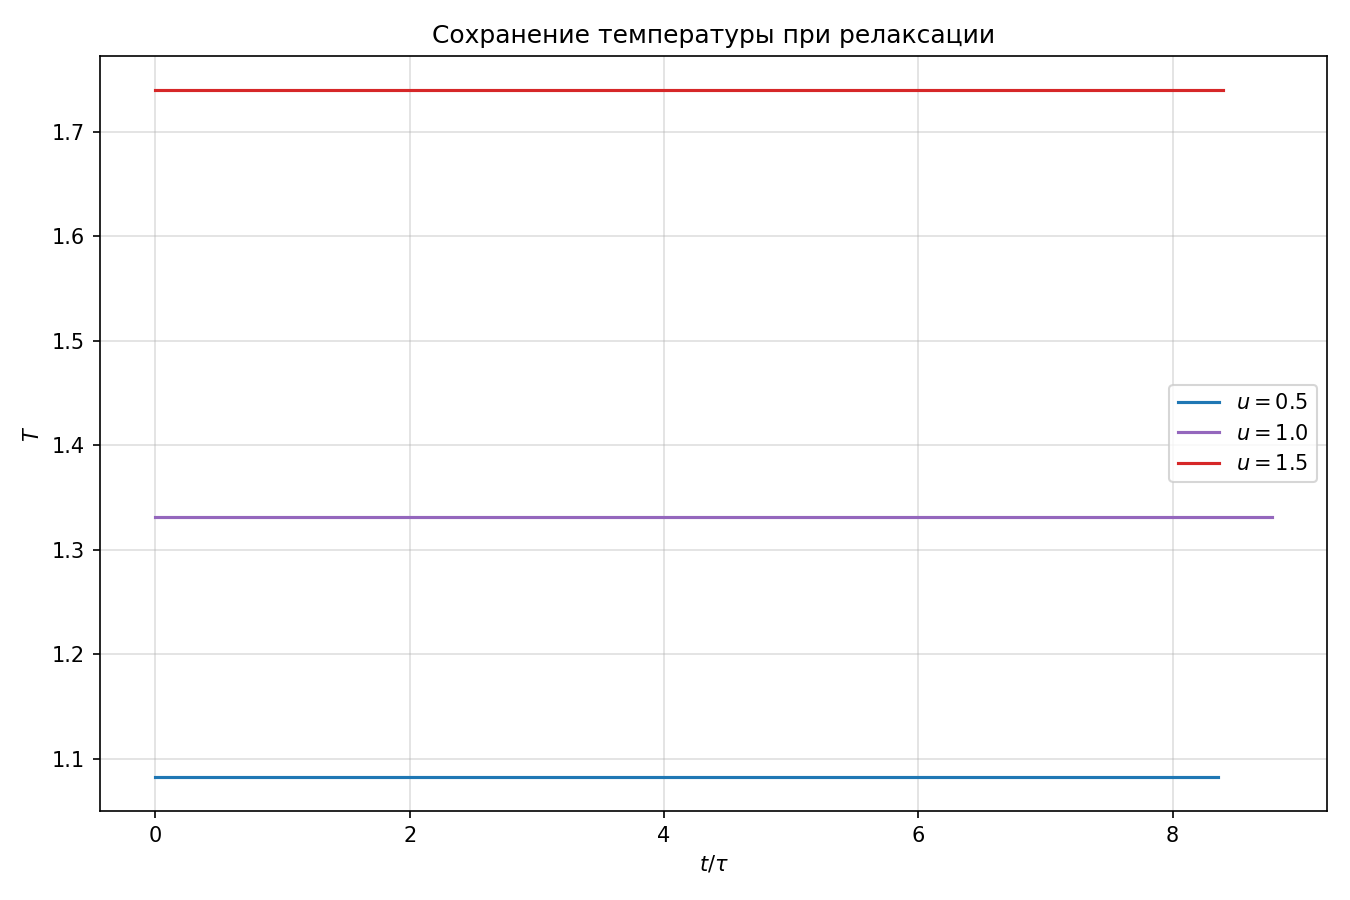
\includegraphics[width=0.7\textwidth]{t0_T}
  \caption{Эволюция температуры $T(t)$ для трёх значений $u$: общая температура сохраняется (контроль энергии).}
  \label{fig:t0T}
\end{figure}

\begin{figure}[htbp]
  \centering
  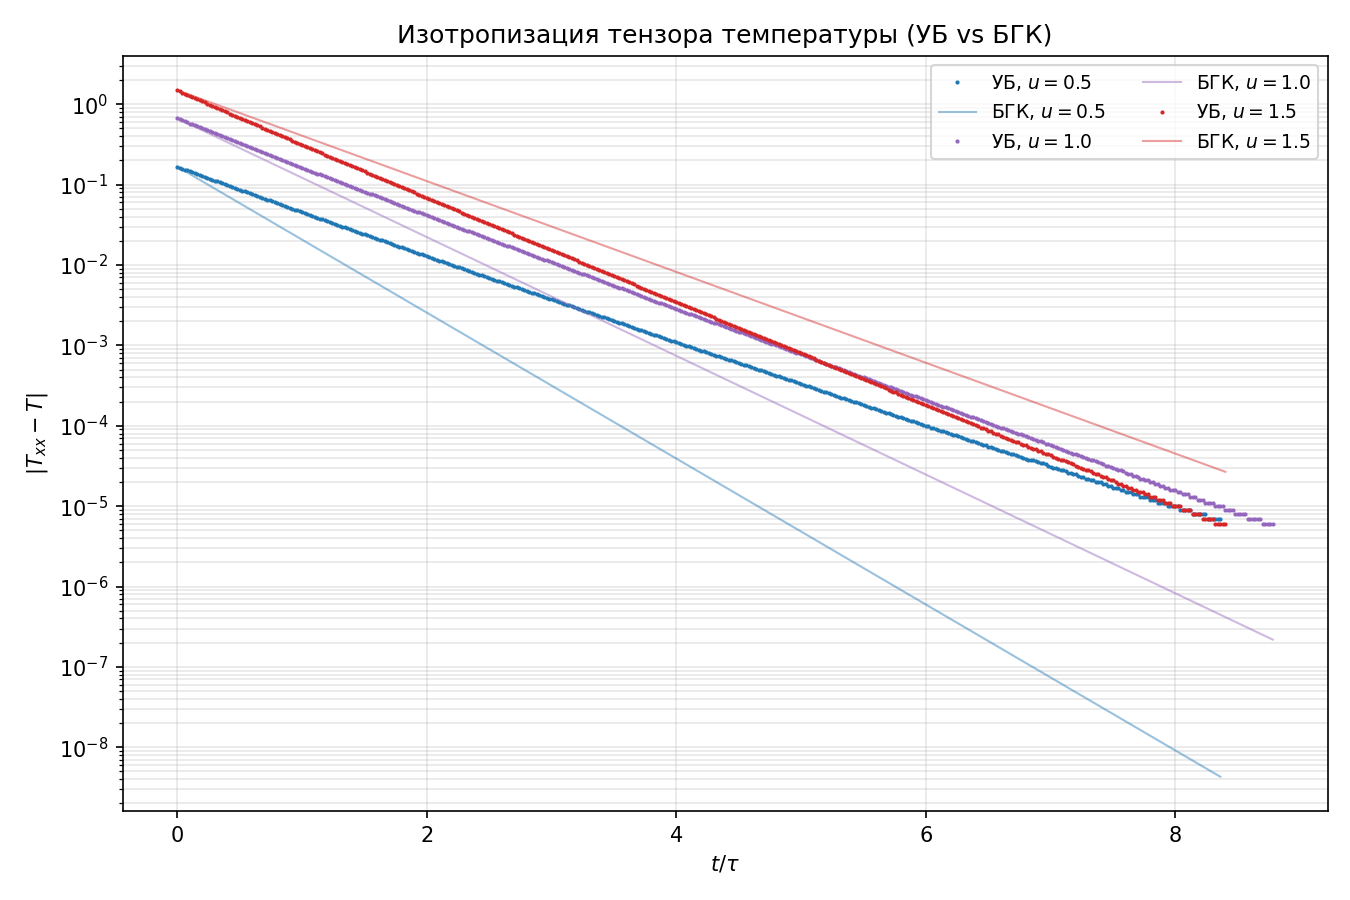
\includegraphics[width=0.7\textwidth]{t0_aniso}
  \caption{Затухание анизотропии $|T_{xx}-T|$ в логарифмическом масштабе в сравнении с моделью БГК.}
  \label{fig:t0aniso}
\end{figure}

\begin{figure}[htbp]
  \centering
  
\includegraphics[width=0.7\textwidth]{t0_H}
  \caption{Эволюция $H$-функции Больцмана: монотонное невозрастание ($H$-теорема).}
  \label{fig:t0H}
\end{figure}

Для интерпретации результат сравнивался с модельным уравнением Бхатнагара--Гросса--Крука (БГК), которое в линейном
режиме даёт экспоненциальную релаксацию $f(t)=f_M+(f(0)-f_M)\,e^{-t/t_{\mathrm{rel}}}$ с единым временем релаксации.
Для модели твёрдых сфер в принятой нормировке при опорном состоянии ($n=1$, $T=1$) оно составляет~\cite{Tcher}
\begin{equation}
  t_{\mathrm{rel}}=\frac{5\sqrt{2}}{16}\approx0{,}442.
\end{equation}
Удобной мерой служит продольный момент четвёртого порядка $M_{xxxx}=\frac1n\sum_\alpha\xi_{x,\alpha}^4 f_\alpha\Delta
V$, равный в равновесии $3T^2$.
Как видно из рис.~\ref{fig:t0m4}, модель БГК с одним временем релаксации упрощает многомодовую структуру реального
оператора столкновений: моменты разных порядков релаксируют со своими скоростями, и наблюдаемое затухание анизотропии
оказывается в среднем медленнее экспоненты БГК, причём на ранних временах для больших $u$ кривая может вести себя
немонотонно.

\begin{figure}[htbp]
  \centering
  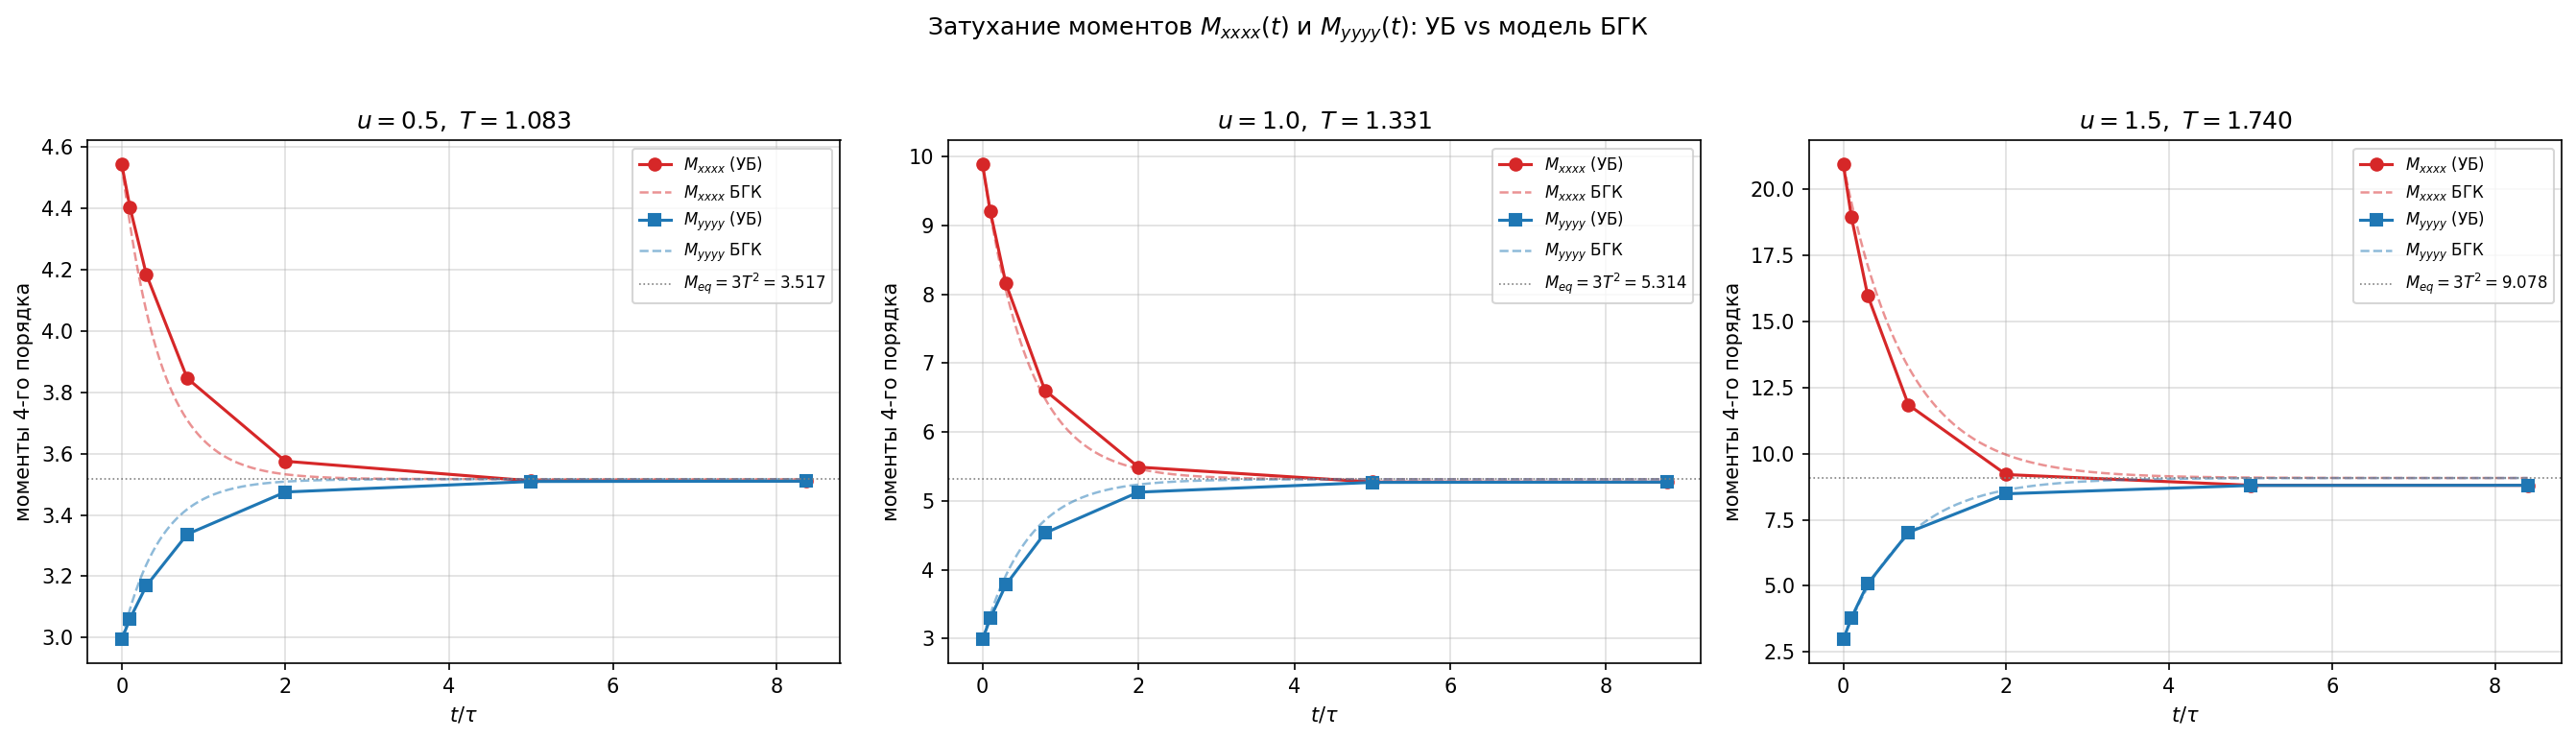
\includegraphics[width=\textwidth]{t0_m4}
\caption{Продольный $M_{xxxx}$ и поперечный $M_{yyyy}$ моменты 4-го порядка: многомодовость релаксации против модели БГК
(пунктир).}
  \label{fig:t0m4}
\end{figure}

Наконец, эволюция одномерной функции распределения $f_x(\xi_x)=\iint f\dd\xi_y\dd\xi_z$ (рис.~\ref{fig:t0fmarg})
наглядно показывает переход от двугорбого распределения (два пика на $\xi_x=\pm u$~--- две встречные «максвелловские
горки») к одногорбому симметричному распределению с максимумом в нуле, то есть к равновесному Максвеллу.
Усреднение по поперечным компонентам опирается на симметрию и подавляет численный шум.

\begin{figure}[htbp]
  \centering
  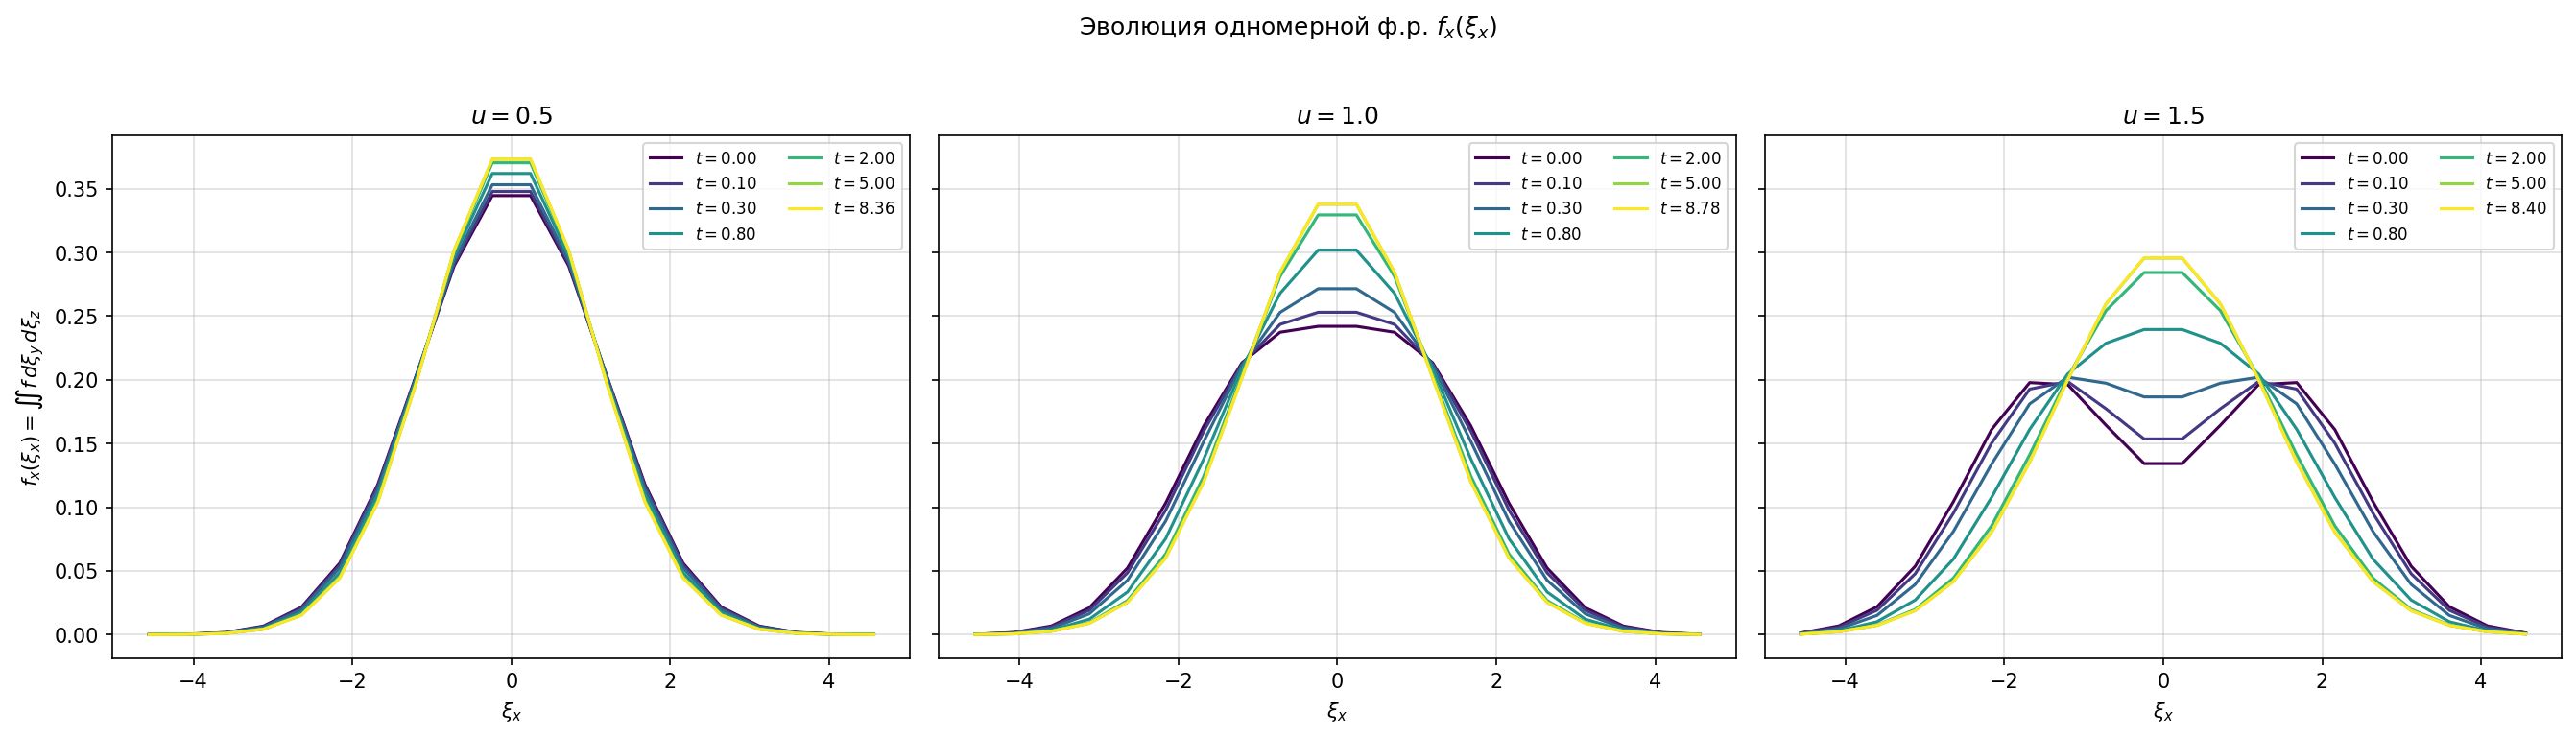
\includegraphics[width=0.95\textwidth]{t0_fmarg}
  \caption{Эволюция одномерной функции распределения $f_x(\xi_x)$ от двугорбой к равновесной максвелловской.}
  \label{fig:t0fmarg}
\end{figure}

Количественная сводка расчёта приведена в табл.~\ref{tab:t0}.
Для всех трёх значений $u$ общая температура $T$ совпадает с установившимся значением $T_{xx}$ (контроль энергии),
$H$-функция убывает, а доля пропущенных по положительности точек равна нулю~--- алгоритм устойчив при выбранных $\tau$ и
$p$.

\begin{table}[h]
  \centering
\caption{Сводка по релаксации квази-шока: число шагов до сходимости, продольная компонента $T_{xx}$ в начале и конце,
равновесная температура $T$ и значения $H$-функции.}
  \label{tab:t0}
  \begin{tabular}{cccccc}
    \hline
    $u$ & Шагов & $T_{xx}$ (старт) & $T_{xx}$ (конец) & $T$ & $H$: старт\,$\to$\,конец\\
    \hline
    0,5 & 419 & 1,249 & 1,083 & 1,083 & $-4{,}367\to-4{,}376$\\
    1,0 & 440 & 1,995 & 1,331 & 1,331 & $-4{,}591\to-4{,}685$\\
    1,5 & 421 & 3,225 & 1,740 & 1,740 & $-4{,}773\to-5{,}083$\\
    \hline
  \end{tabular}
\end{table}

\section{Релаксация бинарной смеси}

Вторая задача~--- релаксация пространственно-однородной смеси двух одноатомных газов с равными концентрациями
$n_c=n_h=0{,}5$ и максвелловскими начальными распределениями, температуры которых различаются вдвое: «холодный» газ
$T_c=1$ и «горячий» $T_h=2$.
Каждая компонента эволюционирует под действием интеграла столкновений со всей смесью $f=f_c+f_h$; требуется вычислить
общую и парциальные температуры, концентрации и энтропии.
Сетка скоростей выбрана крупнее, чтобы захватить тепловой хвост горячей компоненты: $N=28$, $\xi_{\mathrm{cut}}=7{,}0$.

Установившаяся температура смеси есть
\begin{equation}
  T_{\mathrm{eq}}=\frac{n_c T_c+n_h T_h}{n_c+n_h}=1{,}5,
\end{equation}
и расчёт воспроизводит это значение: парциальные температуры монотонно сближаются к общему значению
(рис.~\ref{fig:t1T}), концентрации компонент сохраняются с точностью округления $n_c=n_h=0{,}5$ (рис.~\ref{fig:t1n})~---
прямой контроль работы метода, а суммарная энтропия $S=-\sum f\ln f\,\Delta V$ монотонно возрастает
(рис.~\ref{fig:t1S}).
При этом холодный газ нагревается (его энтропия растёт), а горячий остывает (его энтропия убывает), тогда как энтропия
смеси в целом растёт, достигая максимума в равновесии~--- в согласии со вторым началом термодинамики.
Расчёт выполнен за 310 шагов по времени; доля пропущенных по положительности столкновений практически нулевая.

\begin{figure}[htbp]
  \centering
  
\includegraphics[width=0.7\textwidth]{t1_T}
  \caption{Выравнивание парциальных температур $T_c$ и $T_h$ к общему значению $T_{\mathrm{eq}}=1{,}5$.}
  \label{fig:t1T}
\end{figure}

\begin{figure}[htbp]
  \centering
  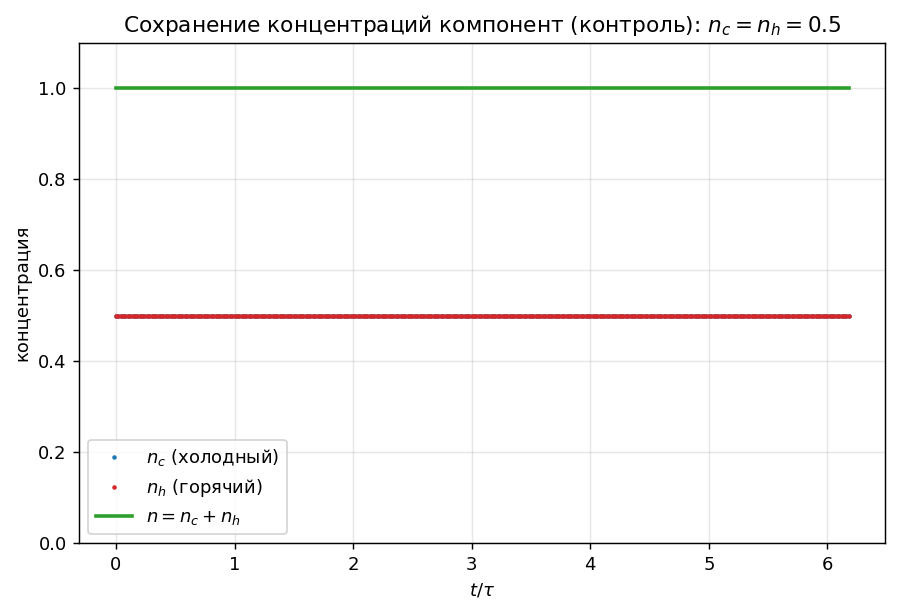
\includegraphics[width=0.7\textwidth]{t1_n}
  \caption{Сохранение концентраций компонент $n_c=n_h=0{,}5$ (контроль метода).}
  \label{fig:t1n}
\end{figure}

\begin{figure}[htbp]
  \centering
  
\includegraphics[width=0.7\textwidth]{t1_S}
  \caption{Энтропии: суммарная энтропия смеси монотонно возрастает ($H$-теорема); компоненты ведут себя противоположно.}
  \label{fig:t1S}
\end{figure}

Количественная сводка приведена в табл.~\ref{tab:t1}: парциальные температуры сходятся к общему значению $T=1{,}5$,
концентрации компонент сохраняются точно, а суммарная энтропия монотонно растёт.

\begin{table}[h]
  \centering
\caption{Сводка по релаксации смеси: парциальные и общая температуры, концентрации и суммарная энтропия в начальный и
конечный (равновесный) моменты.}
  \label{tab:t1}
  \begin{tabular}{lcc}
    \hline
    Величина & $t=0$ & равновесие\\
    \hline
    $T_c$ (холодный газ) & 1,000 & 1,500\\
    $T_h$ (горячий газ)  & 2,000 & 1,500\\
    $T$ (смесь)          & 1,500 & 1,500\\
    $n_c=n_h$            & 0,500 & 0,500\\
    $S$ (смесь)          & 4,855 & 4,865\\
    \hline
  \end{tabular}
\end{table}

Совокупность результатов Главы~2~--- точное сохранение инвариантов, монотонность $H$-функции, установление равновесного
распределения Максвелла и правильное равновесие смеси~--- подтверждает корректность реализованного солвера и позволяет
применить его к неоднородной задаче переноса.



% !TeX root = ../thesis.tex
% ===================== ГЛАВА 3 =====================
\chapter{Задача переноса: ударная волна перед поршнем}

\section{Постановка задачи}

Рассматривается задача о поршне в полупространстве $x\le 0$.
В системе отсчёта, связанной с поршнем, стенка покоится при $x=0$, а слева ($x=-L$) втекает сверхзвуковой поток газа со
скоростью $u_0$.
Скорость потока превышает скорость звука $c=\sqrt{\gamma T}\approx 1{,}291$ (одноатомный газ, $\gamma=5/3$); принято
$u_0=2c\approx 2{,}58$, что отвечает числу Маха набегающего потока $M=u_0/c=2$.
Перед поршнем формируется ударная волна, распространяющаяся в отрицательном направлении.
Эволюция описывается одномерным по пространству и трёхмерным по скоростям уравнением Больцмана
% FIX: в описании задачи в task2/docs/task.txt на строке 14 указано, что задача одномерная
\begin{equation}
  \frac{\partial f}{\partial t}+\xi_x\frac{\partial f}{\partial x}=I(f,f),\qquad f=f(x,\xv,t).
\end{equation}
На стенке задаётся зеркальное (адиабатическое) отражение, слева~--- набегающее максвелловское распределение с дрейфом
$u_0$.

Выбор системы отсчёта, связанной с поршнем, удобен тем, что стенка неподвижна, а расчётная область $[-L,0]$ фиксирована
во времени.
Размер области $L$~--- существенный параметр задачи: фронт ударной волны движется влево со скоростью $V$, и за время
счёта он не должен достигать левой границы; кроме того, область должна вмещать кинетический предвестник~--- сравнительно
быстрые молекулы, уходящие вверх по потоку перед фронтом.
Дискретизация по пространству равномерная, $x_i=-L+(i-\tfrac12)h$ и $h=L/N_x$; по скоростям используется та же сетка с
обрезанием, что и в задачах релаксации. % FIX: так, а в каких пределах меняется i?

\section{Схема расщепления и оператор переноса}

Применяется расщепление Странга по физическим процессам (2-й порядок по времени)
\begin{equation}
  \text{Перенос}\Big(\tfrac{\Delta t}{2}\Big)\;\to\;
  \text{Столкновения}(\Delta t)\;\to\;
  \text{Перенос}\Big(\tfrac{\Delta t}{2}\Big).
\end{equation}
Оператор столкновений совпадает с описанным в главе~1, но в неоднородной задаче выделена лишь поперечная симметрия
(по $\xi_y,\xi_z$): ось $x$ выделена направлением течения, поэтому индекс $\xi_x$ не отражается, что даёт 4-кратную
(а не 8-кратную) связь узлов.
Геометрия столкновений (узлы интерполяции, веса $r_\nu$, модули $|\gv_\nu|$) вычисляется один раз и затем векторно
применяется ко всем пространственным ячейкам.

Оператор переноса $\partial f/\partial t+\xi_x\,\partial f/\partial x=0$ решается монотонной разностной схемой TVD
второго порядка в потоковой форме с ограничителем наклонов MC (monotonic central),
\begin{equation}
  \varphi(\theta)=\max\!\big[0,\ \min(2\theta,\ \tfrac{1+\theta}{2},\ 2)\big],
\end{equation}
для каждого скоростного узла со своим числом Куранта $\nu_a=|\xi_{x}|\,\Delta t/h\le 1$.
% FIX: является ли такое обозначение стандартным? как будто в Пособиях было другое
Граничные условия реализованы через слои фиктивных ячеек: слева~--- набегающий максвелл $f_\infty$ с дрейфом $u_0$,
справа~--- зеркальное отражение (узел $\xi_x\to-\xi_x$), дающее точный отражённый поток.

\section{Теория ударной волны}

Параметры установившейся ударной волны даёт теория Ренкина--Гюгонио.
Для принятых условий число Маха \emph{самого скачка} $M_s\neq M$ набегающего потока и составляет $M_s=3{,}0$; при этом
гидродинамические скачки плотности и температуры равны
% FIX: напомни мне, почему $M_s\neq M$, откуда такие скачки
\begin{equation}
  \frac{n_1}{n_0}=3{,}0,\qquad \frac{T_1}{T_0}\approx 3{,}66,
\end{equation}
а скорость фронта $V=u_0-M_s\,c\approx-1{,}29$ (фронт движется влево). % FIX: почему тут вычитание?
Число Маха скачка связано со скоростью фронта соотношением $M_s=(u_0-V)/c$; самосогласованное решение задачи
поршень--скачок даёт $V=-c$, откуда $M_s=3$. % FIX: то есть ты сначал определил V через M_s, а потом M_s через v?
Эти величины служат ориентиром для проверки результатов кинетического расчёта.

\section{Результаты}

Окончательный расчёт выполнен в конфигурации, обеспечивающей полное развитие ударной волны: расчётная область $L=80$,
число пространственных ячеек $N_x=400$, сетка скоростей с $N=30$ и $\xi_{\mathrm{cut}}=7{,}5$, простое число сетки
Коробова $p=50021$, счёт до $t=40$ ($2000$ шагов).
% FIX: в чём у нас измеряется время? и что значат эти шаги, это расщепление странга?
Размер области выбран из условия $L\gtrsim 75$ (см.\ ниже): при меньших $L$ кинетический предвестник достигает левой
границы и компрессия «застывает» на $n\approx 2{,}3$, не выходя на гидродинамический предел.

На рис.~\ref{fig:t2prof} приведены профили концентрации $n$, скорости $u_x$, температуры $T$ и продольной компоненты
$T_{xx}$ вдоль оси $x$ в несколько моментов времени.
Чётко виден установившийся фронт ударной волны, движущийся влево; за фронтом газ сжат
(концентрация выходит на $n\approx3$) и нагрет ($T\approx3{,}6$), а скорость в системе поршня падает почти до нуля.
% FIX: за фронтом, то есть в сторону 0 или -inf?
На самом фронте заметен немонотонный «перескок» $T_{xx}$~--- характерный кинетический (неравновесный) признак,
отсутствующий в гидродинамическом описании через уравнение Навье-Стокса.
Рис.~\ref{fig:t2front} показывает траекторию фронта $x_c(t)$: после короткого переходного участка она выходит на прямую,
наклон которой даёт скорость фронта $V\approx-1{,}22$.

Эволюция одномерной функции распределения $f_x(\xi_x)$ в середине области (рис.~\ref{fig:t2fx}) иллюстрирует кинетику
ударного перехода: до прихода фронта здесь наблюдается узкий пик набегающего холодного сверхзвукового потока при
$\xi_x\approx u_0$, а после прохождения фронта распределение уширяется и смещается к $\xi_x\approx0$~--- газ
термализуется в «послескачковое» распределение Максвелла.
Тем самым в одном расчёте видны обе стороны ударной волны: сверхзвуковой набегающий поток и дозвуковой сжатый газ за
фронтом.

\begin{figure}[h]
  \centering
  
\includegraphics[width=0.95\textwidth]{t2_profiles}
\caption{Профили макропараметров $n,\,u_x,\,T,\,T_{xx}$ вдоль оси $x$ в различные моменты времени (установившаяся
ударная волна, конфигурация $L=80$, $N_x=400$).}
  \label{fig:t2prof}
\end{figure}

\begin{figure}[h]
  \centering
  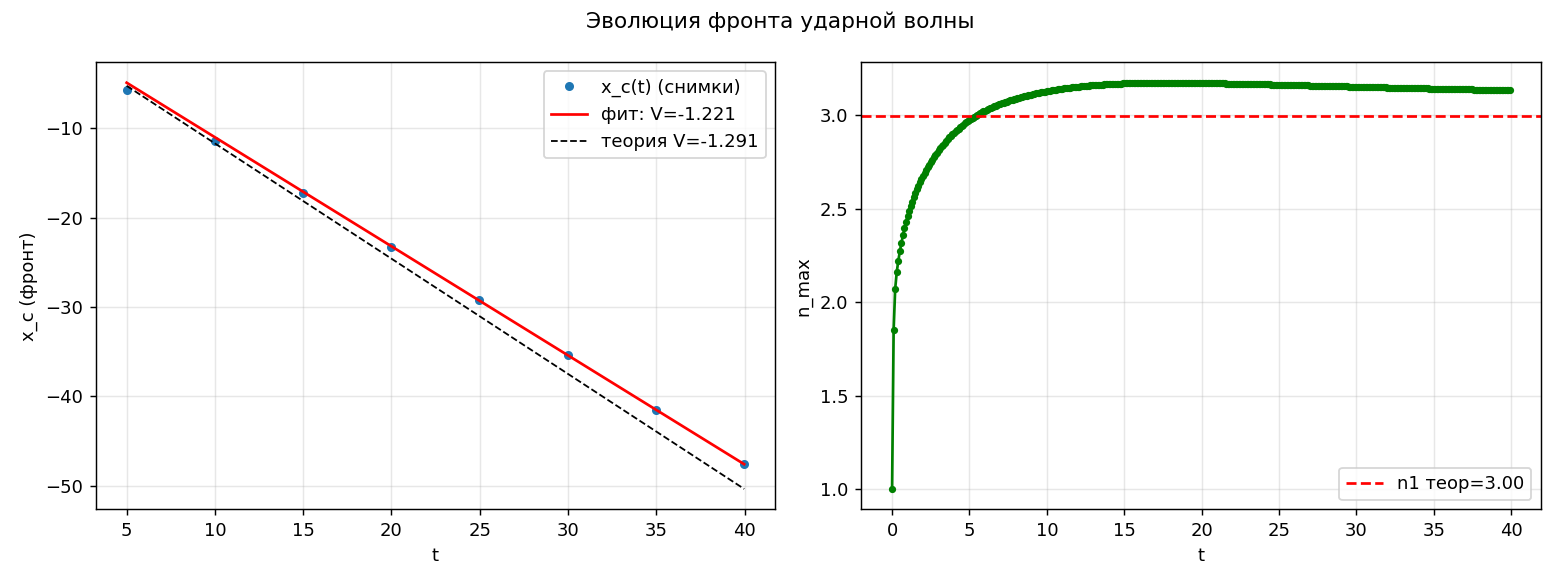
\includegraphics[width=0.8\textwidth]{t2_front}
\caption{Траектория фронта $x_c(t)$ (линейный участок даёт скорость фронта $V$) и эволюция максимальной концентрации
$n_{\max}(t)$.}
  \label{fig:t2front}
\end{figure}

\begin{figure}[h]
  \centering
  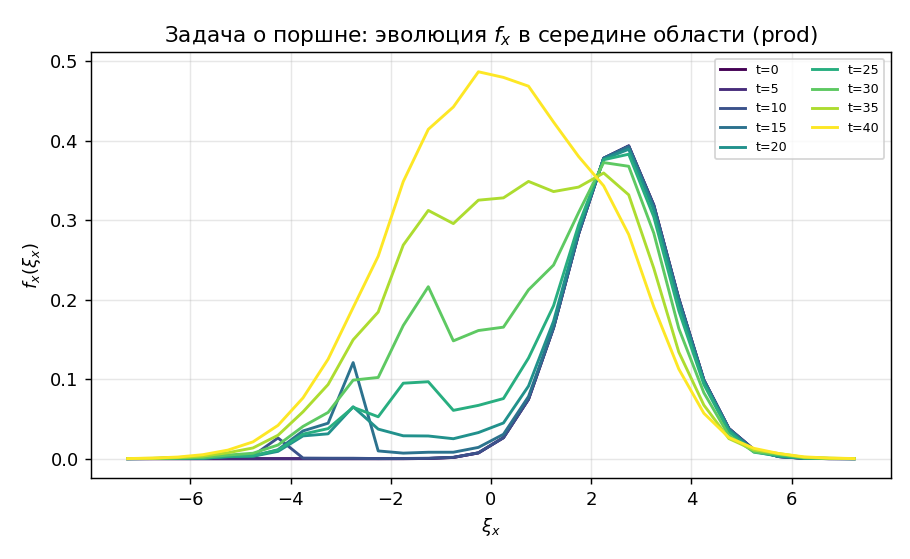
\includegraphics[width=0.8\textwidth]{t2_fx}
\caption{Эволюция $f_x(\xi_x)$ в середине области: переход от холодного набегающего потока (пик при $\xi_x\approx u_0$)
к послескачковому распределению ($\xi_x\approx0$).}
  \label{fig:t2fx}
\end{figure}

\section{Проверка теории Ренкина--Гюгонио}

Сравнение измеренных параметров скачка с точной теорией приведено в табл.~\ref{tab:hugoniot}.
Достигнуто хорошее согласие: скачок плотности $n_1/n_0=2{,}95$ (теория $3{,}0$), скачок температуры $T_1/T_0=3{,}62$
(теория $3{,}66$), скорость фронта $V=-1{,}22$ (теория $-1{,}29$); относительная невязка первого соотношения Гюгонио
$n_0(u_0-V)=n_1(u_1-V)$ составляет $2{,}25\,\%$. % FIX: напомни мне, каков физический смысл этого соотношения?
Масса, импульс и энергия сохраняются с машинной точностью (по построению схемы), а доля пропущенных по условию
положительности точек равна $0{,}53\,\%$~--- в пределах допустимого порога.

\begin{table}[h]
  \centering
\caption{Параметры ударной волны: кинетический расчёт против теории Ренкина--Гюгонио (относительное отклонение вычислено
от неокруглённых значений).}
  \label{tab:hugoniot}
  \begin{tabular}{lccc}
    \hline
    Величина & Расчёт & Теория & Отн.~отклонение\\
    \hline
    Скачок плотности $n_1/n_0$   & 2,954      & 2,999      & 1,5\,\%\\
    Скачок температуры $T_1/T_0$ & 3,617      & 3,663      & 1,3\,\%\\
    Скорость фронта $V$          & $-1{,}221$ & $-1{,}291$ & 5,4\,\%\\
    Число Маха скачка $M_s$      & 2,998      & 3,000      & ---\\
    \hline
  \end{tabular}
\end{table}

Отметим несколько физических особенностей.
% FIX: это строка спряталась между таблицей и графиком и труднозаметна. можно ли её как-то элегантно подвинуть?
Во-первых, выход на гидродинамический скачок $n\to3$ происходит не мгновенно: вблизи стенки сначала формируется
свободномолекулярное удвоение концентрации $n\approx2$ (зеркальное отражение набегающего потока), а затем медленная
компрессия через обратную связь переноса и столкновений доводит концентрацию до $n\approx3$; установившийся режим
достигается к $t\approx10$--$15$.

Во-вторых, ключевую роль играет размер области: за фронтом горячий газ испускает быстрые молекулы вверх по потоку
(кинетический предвестник, вплоть до скоростей $\xi_{\mathrm{cut}}$); если левая граница расположена близко, предвестник
покидает область и компрессия не достигает теоретического значения.
Условие $L\gtrsim\xi_{\mathrm{cut}}\cdot t_{\text{форм}}\approx75$ обеспечивает корректное развитие волны.
В-третьих, несколько большее расхождение по скорости фронта ($5{,}4\,\%$ против $\sim1{,}5\,\%$ по $n$ и $T$) объяснимо:
$V$ извлекается из наклона траектории $x_c(t)$, а фронт имеет конечную кинетическую ширину и чувствителен к порогу его
детектирования. % FIX: что такое кинетическая ширина? чему она равна?
К $t=40$ плато плотности не дошло до $3{,}0$ примерно на $1{,}5\,\%$, что слегка занижает $|V|$.
% FIX: на графике видно, что с ростом времени невязка v растёт. почему так и плохой ли это признак?
Локальные скачки $n$ и $T$ сходятся точнее, тогда как $V$ и интегральная невязка~--- наиболее чувствительные метрики;
% FIX: что здесь является интегральной невязкой?
для кинетического расчёта без подгоночных параметров отклонения в $2$--$5\,\%$~--- хороший результат.
Таким образом, реализованный солвер не только сохраняет инварианты и $H$-функцию, но и количественно воспроизводит
ударно-волновое течение в согласии с теорией.



% !TeX root = ../thesis.tex
% ===================== ГЛАВА 4 =====================
\chapter{Программная реализация и расчёты на суперкомпьютере}

\section{Прототип солвера}

Реализованный солвер представляет собой единую кодовую базу, которая отрабатывает численную схему и проводит тестовые
расчёты задач релаксации и переноса.
Текущая реализация~--- исследовательский прототип, предназначенный для отработки и верификации; вопрос промышленного
высокопроизводительного солвера выделен в отдельное направление (см.~\ref{sec:hpcpath}).

\section{Оптимизации, продиктованные размером задачи}

Размер фазовой сетки (порядка $N^3$ узлов по скоростям на каждую из $N_x$ пространственных ячеек) делает ключевыми две
оптимизации.
Во-первых, геометрия столкновений (узлы проекции, веса $r_\nu$, модули относительных скоростей) \emph{предвычисляется}
один раз, после чего вклад в интеграл столкновений набирается векторно по всем ячейкам, что даёт ускорение примерно на
два порядка по сравнению со скалярной реализацией.
Во-вторых, симметрия функции распределения позволяет хранить её «четвертью» (или «восьмой частью») массива, снижая
расход памяти в $4$--$8$ раз.

\section{Расчёты на суперкомпьютерном кластере}

Работа была выполнена с использованием оборудования центра коллективного пользования «Комплекс моделирования и обработки
данных исследовательских установок мега-класса» НИЦ «Курчатовский институт», http://ckp.nrcki.ru/.
Запуск, контроль состояния, просмотр журналов и выгрузка результатов автоматизированы (цикл
\emph{submit\,/\,status\,/\,log\,/\,fetch}).
Для независимых конфигураций использован механизм \emph{job-array}~--- одновременный счёт нескольких задач (например,
трёх значений параметра $u$ в задаче о квази-шоке).
Так, окончательный расчёт задачи о поршне ($N_x=400$, $p=50021$, $2000$ шагов) потребовал порядка $6 \cdot 10^{9}$
вычислений в узлах сетки Коробова.
Такой длительный прогон, необходимый для выхода ударной волны на стационар, на персональной рабочей станции практически
недостижим.

\section{Структурная параллелизуемость}

Алгоритм по своей природе хорошо распараллеливается: интеграл столкновений вычисляется независимо в каждой
пространственной ячейке, а узлы сетки Коробова независимы между собой.
Это позволяет естественно распределять работу по узлам кластера без существенных коммуникаций между ними.
В однородных задачах релаксации распараллеливание тривиально: независимые конфигурации (например, три значения $u$ в
задаче о квази-шоке) считаются одновременно механизмом \emph{job-array}.
В неоднородной задаче переноса естественная декомпозиция~--- по пространственным ячейкам: оператор столкновений в каждой
ячейке независим, а обмен между подобластями требуется только на шаге переноса и ограничен узкими слоями фиктивных ячеек
на границах.
Таким образом, объём межпроцессорных коммуникаций мал по сравнению с объёмом вычислений, что и обеспечивает хорошую
масштабируемость метода на суперкомпьютерных системах.

\section{Путь к промышленному солверу}
\label{sec:hpcpath}

Прямым продолжением работы является промышленная реализация солвера: компилируемый код (C/C++/Fortran) с
распараллеливанием по пространству средствами MPI и по узлам скоростной сетки на графических ускорителях (GPU)


% !TeX root = ../thesis.tex
% ===================== ЗАКЛЮЧЕНИЕ =====================
\chapter*{Заключение}
\addcontentsline{toc}{chapter}{Заключение}

В работе разработан и верифицирован программный солвер для прямого решения кинетического уравнения Больцмана
консервативным проекционным методом Черемисина с вычислением интеграла столкновений на 8-мерных сетках Коробова.
Основные результаты:
\begin{enumerate}
  \item реализована общая численная схема проекционного метода; подтверждено машинно-точное сохранение
        массы, импульса и энергии, положительность функции распределения и невозрастание $H$-функции;
  \item на задаче релаксации квази-шока воспроизведены сохранение температуры, релаксация продольной
        компоненты тензора температуры и установление равновесного распределения Максвелла; показана
        многомодовая структура релаксации в сравнении с моделью БГК;
  \item на задаче релаксации бинарной смеси воспроизведены выравнивание парциальных температур к
        равновесию $T=1{,}5$, сохранение концентраций и монотонный рост суммарной энтропии;
  \item решена неоднородная задача переноса о поршне: получена установившаяся ударная волна, скачки
        плотности и температуры ($n_1/n_0=2{,}95$, $T_1/T_0=3{,}62$) и скорость фронта ($V=-1{,}22$)
        согласуются с теорией Ренкина--Гюгонио (невязка $\sim2\,\%$) при машинно-точном сохранении
        инвариантов;
  \item расчёты выполнены на суперкомпьютерном кластере; показана структурная параллелизуемость метода.
\end{enumerate}

\textbf{План дальнейших исследований.}
Основное направление развития~--- промышленная компилируемая реализация солвера с распараллеливанием средствами MPI и
GPU.
Перспективны также обобщение на смеси с различными массами компонентов и переход от модели твёрдых сфер к более
реалистичным потенциалам межмолекулярного взаимодействия.



% !TeX root = ../thesis.tex
% ===================== СПИСОК ЛИТЕРАТУРЫ =====================
\begin{thebibliography}{9}
\addcontentsline{toc}{chapter}{Список литературы}

\bibitem{LL10} \emph{Лифшиц Е.\,М., Питаевский Л.\,П.} Физическая кинетика.~--- М.: Наука. Гл.~ред.
физ.-мат. лит., 1979.~--- 528~с. (Теоретическая физика, т.~X).

\bibitem{Kogan} \emph{Коган М.\,Н.} Динамика разреженного газа.~--- М.: Наука, 1967.~--- 440~с.

\bibitem{Tcher} \emph{Черемисин Ф.\,Г.} Введение в консервативный проекционный метод вычисления
интеграла столкновений и метод решения уравнения Больцмана: учебное пособие.~--- М.: МФТИ, 2015.~--- 80~с.

\bibitem{Bird} \emph{Bird G.\,A.} Molecular Gas Dynamics and the Direct Simulation of Gas Flows.~---
Oxford: Clarendon Press, 1994.~--- 458~p.

\bibitem{Aristov} \emph{Аристов В.\,В.} Прямые методы решения уравнения Больцмана и изучение неравновесных
течений.~--- М.: Физматлит, 2001.

\bibitem{Korobov} \emph{Коробов Н.\,М.} Теоретико-числовые методы в приближённом анализе.~--- М.:
Физматгиз, 1963.~--- 224~с.

\bibitem{TcherJCP} \emph{Tcheremissine F.\,G.} Solution of the Boltzmann kinetic equation for high speed
flows~// Computational Mathematics and Mathematical Physics.~--- 2006.~--- Vol.~46, no.~2.~--- P.~315--329.
\end{thebibliography}



% !TeX root = ../thesis.tex
% ===================== ПРИЛОЖЕНИЕ =====================
\chapter*{Приложение А. Псевдокод алгоритма}
\addcontentsline{toc}{chapter}{Приложение А. Псевдокод алгоритма}

Ниже приведён язык-независимый псевдокод одного шага по времени (комментарии~--- латиницей, чтобы не зависеть от шрифта
моноширинного блока).

\medskip
\noindent\textbf{Шаг проекционного метода (интеграл столкновений):}
{\footnotesize
\begin{verbatim}
for each time step:
    refresh random shift delta of the Korobov lattice
    for nu = 1 .. p:                  # nodes of the 8D Korobov lattice
        recover (eps, b, xi_a, xi_b) from Korobov coordinates
        if |xi_a| > xi_cut or |xi_b| > xi_cut: skip nu
        theta = 2*arccos(b / b_max)   # hard-sphere model
        g'    = rotate(xi_b - xi_a, theta, eps)
        xi_a' = 0.5*(xi_a + xi_b) - 0.5*g'
        xi_b' = 0.5*(xi_a + xi_b) + 0.5*g'
        (lam, mu, s, r) = project_to_nodes(xi_a', xi_b')  # momentum + energy
        Omega = (f[lam]*f[mu])^(1-r) * (f[lam+s]*f[mu-s])^r - f[a]*f[b]
        df = C * Omega * |g|
        if positivity is violated at any of the 6 nodes: skip nu
        else: apply df to nodes (a, b, lam, mu, lam+s, mu-s)
\end{verbatim}
}

\medskip
\noindent\textbf{Шаг задачи переноса (расщепление Странга):}
{\footnotesize
\begin{verbatim}
transport(dt/2)      # TVD scheme with MC limiter, per velocity node
collisions(dt)       # see pseudocode above
transport(dt/2)
# boundary conditions: left  - incoming Maxwellian f_inf(u0)
#                      right - specular reflection xi_x -> -xi_x
\end{verbatim}
}


\end{document}
